\documentclass[border=2pt]{standalone}
\usepackage{tikz}
\usepackage{pgfplots}
\pgfplotsset{compat=1.18}
\usepgfplotslibrary{fillbetween}

% Brand colors
\definecolor{Garnet}{rgb}{0.451, 0.0, 0.039}
\definecolor{Atlantic}{rgb}{0.275, 0.416, 0.624}
\definecolor{Rose}{rgb}{0.8, 0.18, 0.251}
\definecolor{Black70}{rgb}{0.361, 0.361, 0.361}
\definecolor{Black90}{rgb}{0.212, 0.212, 0.212}

\begin{document}
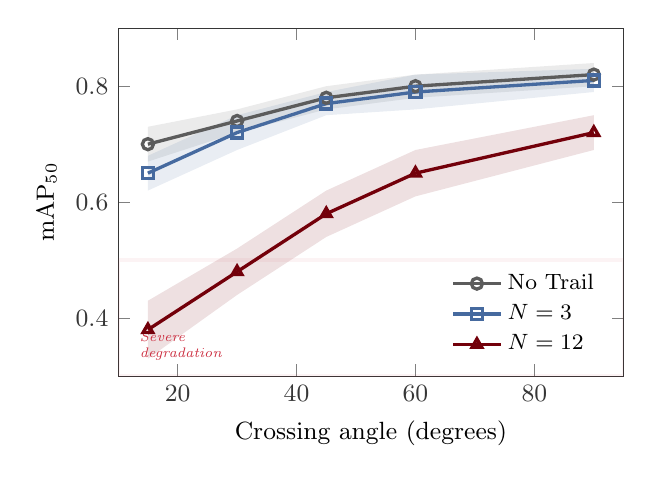
\begin{tikzpicture}
\begin{axis}[
  width=8cm,
  height=6cm,
  xmin=10, xmax=95,
  ymin=0.3, ymax=0.9,
  xlabel={Crossing angle (degrees)},
  ylabel={mAP$_{50}$},
  xlabel style={font=\small},
  ylabel style={font=\small},
  axis line style={Black90},
  tick label style={font=\small, color=Black90},
  legend style={
    at={(0.97,0.03)},
    anchor=south east,
    draw=none,
    fill=none,
    font=\footnotesize,
    cells={anchor=west}
  },
  rounded corners=0pt,
  every axis plot/.append style={line width=1.2pt}
]

% Severe degradation shading
\addplot[Rose, opacity=0.06, forget plot, area legend]
  coordinates {(10,0.3) (95,0.3) (95,0.5) (10,0.5)} \closedcycle;
\node[font=\tiny, color=Rose, anchor=south west, text width=1.2cm, align=left]
  at (axis cs:12,0.31) {\textit{Severe degradation}};

% No Trail
\addplot[color=Black70, mark=o, mark size=2pt]
  coordinates {(15,0.70) (30,0.74) (45,0.78) (60,0.80) (90,0.82)};
\addlegendentry{No Trail}
\addplot[name path=none_upper, draw=none, forget plot]
  coordinates {(15,0.73) (30,0.76) (45,0.80) (60,0.82) (90,0.84)};
\addplot[name path=none_lower, draw=none, forget plot]
  coordinates {(15,0.67) (30,0.72) (45,0.76) (60,0.78) (90,0.80)};
\addplot[Black70, opacity=0.12, forget plot] fill between[of=none_upper and none_lower];

% Short trails N=3
\addplot[color=Atlantic, mark=square, mark size=2pt]
  coordinates {(15,0.65) (30,0.72) (45,0.77) (60,0.79) (90,0.81)};
\addlegendentry{$N=3$}
\addplot[name path=short_upper, draw=none, forget plot]
  coordinates {(15,0.68) (30,0.75) (45,0.79) (60,0.82) (90,0.83)};
\addplot[name path=short_lower, draw=none, forget plot]
  coordinates {(15,0.62) (30,0.69) (45,0.75) (60,0.76) (90,0.79)};
\addplot[Atlantic, opacity=0.12, forget plot] fill between[of=short_upper and short_lower];

% Long trails N=12
\addplot[color=Garnet, mark=triangle, mark size=2pt]
  coordinates {(15,0.38) (30,0.48) (45,0.58) (60,0.65) (90,0.72)};
\addlegendentry{$N=12$}
\addplot[name path=long_upper, draw=none, forget plot]
  coordinates {(15,0.43) (30,0.52) (45,0.62) (60,0.69) (90,0.75)};
\addplot[name path=long_lower, draw=none, forget plot]
  coordinates {(15,0.33) (30,0.44) (45,0.54) (60,0.61) (90,0.69)};
\addplot[Garnet, opacity=0.12, forget plot] fill between[of=long_upper and long_lower];

\end{axis}
\end{tikzpicture}
\end{document}
